

% \tikzset{every picture/.style={line width=0.75pt}} %set default line width to 0.75pt        

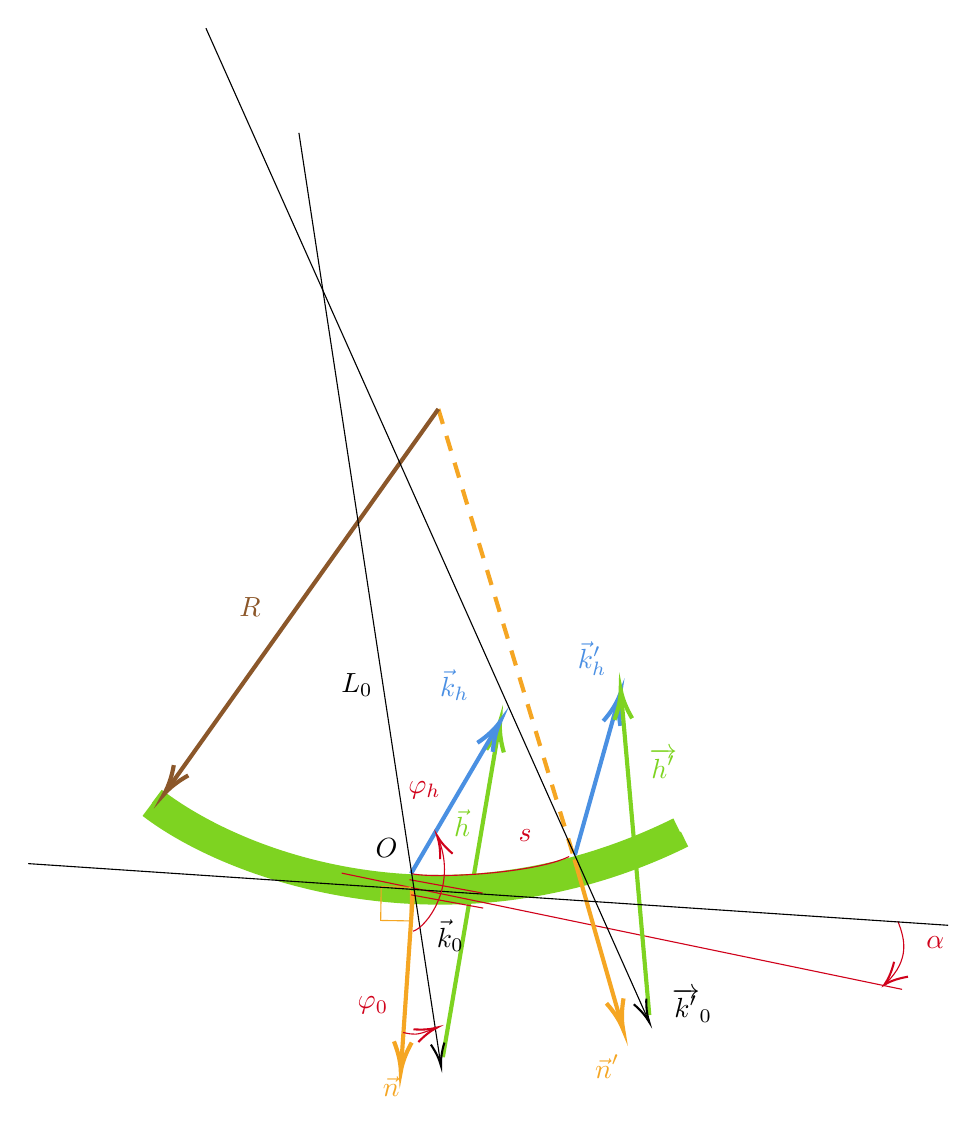
\begin{tikzpicture}[x=0.75pt,y=0.75pt,yscale=-1,xscale=1]
%uncomment if require: \path (0,438); %set diagram left start at 0, and has height of 438

%Curve Lines [id:da5232051232783406] 
\draw [color={rgb, 255:red, 126; green, 211; blue, 33 }  ,draw opacity=1 ][line width=6]    (175.47,272.23) .. controls (219.4,305.82) and (326.96,339.57) .. (434.2,286.6) ;
%Straight Lines [id:da16285737660398936] 
\draw [color={rgb, 255:red, 245; green, 166; blue, 35 }  ,draw opacity=1 ][line width=1.5]    (303.8,306.2) -- (297.71,395.54) ;
\draw [shift={(297.51,398.54)}, rotate = 273.9] [color={rgb, 255:red, 245; green, 166; blue, 35 }  ,draw opacity=1 ][line width=1.5]    (14.21,-4.28) .. controls (9.04,-1.82) and (4.3,-0.39) .. (0,0) .. controls (4.3,0.39) and (9.04,1.82) .. (14.21,4.28)   ;
%Straight Lines [id:da9494728644400778] 
\draw [color={rgb, 255:red, 126; green, 211; blue, 33 }  ,draw opacity=1 ][line width=1.5]    (317.75,391.65) -- (344.81,233.1) ;
\draw [shift={(345.31,230.14)}, rotate = 459.69] [color={rgb, 255:red, 126; green, 211; blue, 33 }  ,draw opacity=1 ][line width=1.5]    (14.21,-4.28) .. controls (9.04,-1.82) and (4.3,-0.39) .. (0,0) .. controls (4.3,0.39) and (9.04,1.82) .. (14.21,4.28)   ;
%Curve Lines [id:da9991370331234093] 
\draw [color={rgb, 255:red, 126; green, 211; blue, 33 }  ,draw opacity=1 ][line width=6]    (179.93,266.04) .. controls (223.86,299.64) and (323.35,333.23) .. (430.58,280.26) ;
%Straight Lines [id:da5249374072906461] 
\draw [color={rgb, 255:red, 208; green, 2; blue, 27 }  ,draw opacity=1 ]   (539,359) -- (269,303) ;
%Straight Lines [id:da1028859118738259] 
\draw [color={rgb, 255:red, 245; green, 166; blue, 35 }  ,draw opacity=1 ][line width=1.5]  [dash pattern={on 5.63pt off 4.5pt}]  (315.59,79.41) -- (381.2,296.4) ;
%Straight Lines [id:da34959262043431627] 
\draw [color={rgb, 255:red, 208; green, 2; blue, 27 }  ,draw opacity=1 ]   (301.98,313.39) -- (337.19,319.85) ;
%Straight Lines [id:da16405055688919945] 
\draw [color={rgb, 255:red, 74; green, 144; blue, 226 }  ,draw opacity=1 ][line width=1.5]    (302.44,303.23) -- (343.79,232.73) ;
\draw [shift={(345.31,230.14)}, rotate = 480.4] [color={rgb, 255:red, 74; green, 144; blue, 226 }  ,draw opacity=1 ][line width=1.5]    (14.21,-4.28) .. controls (9.04,-1.82) and (4.3,-0.39) .. (0,0) .. controls (4.3,0.39) and (9.04,1.82) .. (14.21,4.28)   ;
%Straight Lines [id:da5835744267291234] 
\draw [color={rgb, 255:red, 74; green, 144; blue, 226 }  ,draw opacity=1 ][line width=1.5]    (381.4,294.2) -- (402.21,220.11) ;
\draw [shift={(403.02,217.22)}, rotate = 465.69] [color={rgb, 255:red, 74; green, 144; blue, 226 }  ,draw opacity=1 ][line width=1.5]    (14.21,-4.28) .. controls (9.04,-1.82) and (4.3,-0.39) .. (0,0) .. controls (4.3,0.39) and (9.04,1.82) .. (14.21,4.28)   ;
%Straight Lines [id:da08988888504673165] 
\draw [color={rgb, 255:red, 126; green, 211; blue, 33 }  ,draw opacity=1 ][line width=1.5]    (417.23,371.41) -- (403.71,217.63) ;
\draw [shift={(403.45,214.64)}, rotate = 444.98] [color={rgb, 255:red, 126; green, 211; blue, 33 }  ,draw opacity=1 ][line width=1.5]    (14.21,-4.28) .. controls (9.04,-1.82) and (4.3,-0.39) .. (0,0) .. controls (4.3,0.39) and (9.04,1.82) .. (14.21,4.28)   ;
%Straight Lines [id:da40950439043897857] 
\draw [color={rgb, 255:red, 139; green, 87; blue, 42 }  ,draw opacity=1 ][line width=1.5]    (315.59,79.41) -- (185.12,262.58) ;
\draw [shift={(183.38,265.03)}, rotate = 305.46] [color={rgb, 255:red, 139; green, 87; blue, 42 }  ,draw opacity=1 ][line width=1.5]    (14.21,-4.28) .. controls (9.04,-1.82) and (4.3,-0.39) .. (0,0) .. controls (4.3,0.39) and (9.04,1.82) .. (14.21,4.28)   ;
%Curve Lines [id:da5639281109914969] 
\draw [color={rgb, 255:red, 208; green, 2; blue, 27 }  ,draw opacity=1 ]   (536.96,326.18) .. controls (540.68,335.28) and (542.42,344.77) .. (531.88,355.42) ;
\draw [shift={(530.5,356.76)}, rotate = 317.12] [color={rgb, 255:red, 208; green, 2; blue, 27 }  ,draw opacity=1 ][line width=0.75]    (10.93,-4.9) .. controls (6.95,-2.3) and (3.31,-0.67) .. (0,0) .. controls (3.31,0.67) and (6.95,2.3) .. (10.93,4.9)   ;
%Curve Lines [id:da42206687748786953] 
\draw [color={rgb, 255:red, 208; green, 2; blue, 27 }  ,draw opacity=1 ]   (378.6,295) .. controls (362.23,303.18) and (313.2,305.81) .. (302.44,303.23) ;
%Straight Lines [id:da2409863293898824] 
\draw [color={rgb, 255:red, 208; green, 2; blue, 27 }  ,draw opacity=1 ]   (301.7,306.16) -- (336.91,312.62) ;
%Straight Lines [id:da06706363543945182] 
\draw [color={rgb, 255:red, 245; green, 166; blue, 35 }  ,draw opacity=1 ][line width=1.5]    (381.2,296.4) -- (403.77,375.32) ;
\draw [shift={(404.6,378.2)}, rotate = 254.04000000000002] [color={rgb, 255:red, 245; green, 166; blue, 35 }  ,draw opacity=1 ][line width=1.5]    (14.21,-4.28) .. controls (9.04,-1.82) and (4.3,-0.39) .. (0,0) .. controls (4.3,0.39) and (9.04,1.82) .. (14.21,4.28)   ;
%Shape: Rectangle [id:dp16408028713981904] 
\draw  [color={rgb, 255:red, 245; green, 166; blue, 35 }  ,draw opacity=1 ] (288.07,309.57) -- (302.21,309.8) -- (301.94,326.03) -- (287.8,325.8) -- cycle ;
%Straight Lines [id:da6014347424725826] 
\draw [color={rgb, 255:red, 0; green, 0; blue, 0 }  ,draw opacity=1 ]   (561.16,328.14) -- (118,298.43) ;
%Straight Lines [id:da19735589184858027] 
\draw    (248.41,-53.67) -- (316.58,393.98) ;
\draw [shift={(316.89,395.95)}, rotate = 261.34000000000003] [color={rgb, 255:red, 0; green, 0; blue, 0 }  ][line width=0.75]    (10.93,-3.29) .. controls (6.95,-1.4) and (3.31,-0.3) .. (0,0) .. controls (3.31,0.3) and (6.95,1.4) .. (10.93,3.29)   ;
%Straight Lines [id:da01862679429167091] 
\draw    (203.62,-104.06) -- (416.42,373.02) ;
\draw [shift={(417.23,374.85)}, rotate = 245.95999999999998] [color={rgb, 255:red, 0; green, 0; blue, 0 }  ][line width=0.75]    (10.93,-3.29) .. controls (6.95,-1.4) and (3.31,-0.3) .. (0,0) .. controls (3.31,0.3) and (6.95,1.4) .. (10.93,3.29)   ;
%Curve Lines [id:da6524290863430278] 
\draw [color={rgb, 255:red, 208; green, 2; blue, 27 }  ,draw opacity=1 ]   (313.1,378.13) .. controls (304.57,381.34) and (304.21,380.92) .. (298.6,379.8) ;
\draw [shift={(315,377.4)}, rotate = 158.96] [color={rgb, 255:red, 208; green, 2; blue, 27 }  ,draw opacity=1 ][line width=0.75]    (10.93,-3.29) .. controls (6.95,-1.4) and (3.31,-0.3) .. (0,0) .. controls (3.31,0.3) and (6.95,1.4) .. (10.93,3.29)   ;
%Curve Lines [id:da985679797920541] 
\draw [color={rgb, 255:red, 208; green, 2; blue, 27 }  ,draw opacity=1 ]   (315.87,287.08) .. controls (324.5,309.43) and (310,329.06) .. (303.4,331) ;
\draw [shift={(315,285)}, rotate = 65.85] [color={rgb, 255:red, 208; green, 2; blue, 27 }  ,draw opacity=1 ][line width=0.75]    (10.93,-3.29) .. controls (6.95,-1.4) and (3.31,-0.3) .. (0,0) .. controls (3.31,0.3) and (6.95,1.4) .. (10.93,3.29)   ;

% Text Node
\draw (284.13,284.95) node [anchor=north west][inner sep=0.75pt]   [align=left] {$\displaystyle O$};
% Text Node
\draw (549.48,332.26) node [anchor=north west][inner sep=0.75pt]   [align=left] {$\displaystyle \textcolor[rgb]{0.82,0.01,0.11}{\alpha }$};
% Text Node
\draw (313.65,324.31) node [anchor=north west][inner sep=0.75pt]   [align=left] {$\displaystyle \vec{k}_{0}$};
% Text Node
\draw (267.55,205.64) node [anchor=north west][inner sep=0.75pt]   [align=left] {$\displaystyle L_{0}$};
% Text Node
\draw (321.94,271.12) node [anchor=north west][inner sep=0.75pt]  [color={rgb, 255:red, 126; green, 211; blue, 33 }  ,opacity=1 ] [align=left] {$\displaystyle \vec{\textcolor[rgb]{0.49,0.83,0.13}{h}}$};
% Text Node
\draw (381.5,190.34) node [anchor=north west][inner sep=0.75pt]   [align=left] {$\displaystyle \textcolor[rgb]{0.29,0.56,0.89}{\vec{k} '_{h}}$};
% Text Node
\draw (426.91,357.26) node [anchor=north west][inner sep=0.75pt]   [align=left] {$\displaystyle \overrightarrow{k'}_{0}$};
% Text Node
\draw (287.56,399.74) node [anchor=north west][inner sep=0.75pt]   [align=left] {$\displaystyle \textcolor[rgb]{0.96,0.65,0.14}{\vec{\textcolor[rgb]{0.96,0.65,0.14}{n}}}$};
% Text Node
\draw (389.85,389.4) node [anchor=north west][inner sep=0.75pt]   [align=left] {$\displaystyle \textcolor[rgb]{0.96,0.65,0.14}{\vec{\textcolor[rgb]{0.96,0.65,0.14}{n}} '}$};
% Text Node
\draw (315.21,203.51) node [anchor=north west][inner sep=0.75pt]   [align=left] {$\displaystyle \textcolor[rgb]{0.29,0.56,0.89}{\vec{k}_{h}}$};
% Text Node
\draw (415.98,241.83) node [anchor=north west][inner sep=0.75pt]  [color={rgb, 255:red, 126; green, 211; blue, 33 }  ,opacity=1 ] [align=left] {$\displaystyle \overrightarrow{\textcolor[rgb]{0.49,0.83,0.13}{h'}}$};
% Text Node
\draw (218.44,169.03) node [anchor=north west][inner sep=0.75pt]   [align=left] {$\displaystyle \textcolor[rgb]{0.55,0.34,0.16}{R}$};
% Text Node
\draw (352.95,280.58) node [anchor=north west][inner sep=0.75pt]   [align=left] {$\displaystyle \textcolor[rgb]{0.82,0.01,0.11}{s}$};
% Text Node
\draw (275.48,361.46) node [anchor=north west][inner sep=0.75pt]   [align=left] {$\displaystyle \textcolor[rgb]{0.82,0.01,0.11}{\varphi _{0}}$};
% Text Node
\draw (299.88,257.46) node [anchor=north west][inner sep=0.75pt]   [align=left] {$\displaystyle \textcolor[rgb]{0.82,0.01,0.11}{\varphi }\textcolor[rgb]{0.82,0.01,0.11}{_{h}}$};


\end{tikzpicture}
